\documentclass[11pt]{article}
%\usepackage[firstpage]{draftwatermark}
\usepackage{times}
\usepackage{pdfpages}
\usepackage{fullpage}
\usepackage{url}
\usepackage{hyperref}
\usepackage{fancyhdr}
\usepackage{graphicx}
\usepackage{tabularx}
\usepackage{enumitem}
\usepackage{indentfirst}
\usepackage{subcaption}

% Added by bsb
\usepackage{color,soul}
\DeclareRobustCommand{\hlr}[1]{{\sethlcolor{red}\hl{#1}}}
\DeclareRobustCommand{\hlg}[1]{{\sethlcolor{green}\hl{#1}}}
\DeclareRobustCommand{\hlb}[1]{{\sethlcolor{blue}\hl{#1}}}
\DeclareRobustCommand{\hly}[1]{{\sethlcolor{yellow}\hl{#1}}}


\setcounter{secnumdepth}{4}
\graphicspath{{images/}}
\pagestyle{fancy}

% Conditional for notes
\newif\ifnotes
\notesfalse


\newcommand{\proposaltitle}{Wave Spectra Notes}

\newcommand{\proposalnumber}{\proposaltitle}

\addtolength{\headheight}{2em}
\addtolength{\headsep}{1.5em}
\lhead{\proposalnumber}
\rhead{}

\newcommand{\capt}[1]{\caption{\small \em #1}}

\cfoot{\small Brian Bingham \today \\ \thepage}
\renewcommand{\footrulewidth}{0.4pt}

\newenvironment{xitemize}{\begin{itemize}\addtolength{\itemsep}{-0.75em}}{\end{itemize}}
\newenvironment{tasklist}{\begin{enumerate}[label=\textbf{\thesubsubsection-\arabic*},ref=\thesubsubsection-\arabic*,leftmargin=*]}{\end{enumerate}}
\newcommand\todo[1]{{\bf TODO: #1}}
\setcounter{tocdepth}{2}
\setcounter{secnumdepth}{4}

\makeatletter
\newcommand*{\compress}{\@minipagetrue}
\makeatother

%\renewcommand{\chaptername}{Volume}
%\renewcommand{\thesection}{\Roman{section}}
%\renewcommand{\thesubsection}{\Roman{section}-\Alph{subsection}}

\begin{document}
%\thispagestyle{empty}
% Project Summary
\section*{Project Summary}
Lorem ipsum dolor sit amet, consectetur adipiscing elit. Pellentesque sit amet posuere mi. Etiam pretium ipsum massa. Curabitur dignissim quam in semper suscipit. Morbi sodales diam consequat ex euismod cursus. Curabitur cursus ligula eget nisi fermentum imperdiet. Nam commodo massa eget nisl lobortis, vel consequat sem gravida. Sed turpis lorem, aliquet sed ultricies eu, pharetra consectetur odio. Curabitur id iaculis dolor. Cras pellentesque lectus ac ex elementum hendrerit. Ut fermentum velit vitae ipsum elementum cursus. Aenean imperdiet, dolor eleifend rutrum pulvinar, tortor leo varius risus, eu pulvinar lectus nunc eget ligula. Aliquam vitae laoreet massa \cite{cook14survey}.

\newpage
% Title Page
\setcounter{page}{1}
\begin{center}

\vspace*{0.25in}

{\Large ONR Proposal}

\vspace*{0.25in}

{\huge \proposaltitle}

\vspace*{0.5in}
\renewcommand{\arraystretch}{2.0}
\begin{tabular}{|p{1.5in}|p{2.5in}|} \hline
Investigator: & 
  Brian Bingham \newline
  Associate Professor \newline
  Mechanical and Aerospace Engineering Department \newline
  Naval Postgraduate School  \newline
  700 Dyer Rd, Watkins 331  \newline
  Monterey, CA 93943  \newline
  Office: (831) 656-2396  \newline
  Email: bsbingha@nps.edu  \newline
\\ \hline
To: & Kelly Cooper, ONR Code 33 
\\ \hline
Project Duration: & Two Years, FY2018-FY2019 
\\ \hline
 
\end{tabular}
\end{center}
\vspace*{\fill}
\pagebreak

\ifnotes
\begin{itemize}
\item Notes/requests for Brian G. (BG) are in \hlg{green}
\item Notes/requests for Brian B. (BB)are in \hlr{red}
\item General notes are in \hly{yellow}
\end{itemize}
\fi

\section{Long Term Goals}
Lorem ipsum dolor sit amet, consectetur adipiscing elit. Pellentesque sit amet posuere mi. Etiam pretium ipsum massa. Curabitur dignissim quam in semper suscipit. Morbi sodales diam consequat ex euismod cursus. Curabitur cursus ligula eget nisi fermentum imperdiet. Nam commodo massa eget nisl lobortis, vel consequat sem gravida. Sed turpis lorem, aliquet sed ultricies eu, pharetra consectetur odio. Curabitur id iaculis dolor. Cras pellentesque lectus ac ex elementum hendrerit. Ut fermentum velit vitae ipsum elementum cursus. Aenean imperdiet, dolor eleifend rutrum pulvinar, tortor leo varius risus, eu pulvinar lectus nunc eget ligula. Aliquam vitae laoreet massa.


\section{Research Objectives}
We propose to create an authentic, open-source virtual robotics environment to accelerate the development and evaluation of ocean robotics and to use these tools to create and host the 2019 Virtual Maritime RobotX Challenge (VMRC).  In the near-term this infrastructure will support the RobotX challenge, complementing the ongoing series of RobotX competitions.  However, as demonstrated by past virtual robotics competitions, development of foundational simulation capabilities has a lasting benefit beyond the competition itself.  The simulation environment would be immediately useful for participants in similar events such as RoboBoat and RoboSub.   Also, by extending the Gazebo simulation environment to enable multi-domain vehicle coordination (under, at and over the water surface), we will provide a common, accessible, authentic basis for rapid design and testing of robotic platforms in the complex ocean environment beyond competition applications.

The goals of this project are to
\begin{xitemize}
\item Lorem ipsum dolor sit amet, consectetur adipiscing elit.
\item Aliquam porta elit sed purus consectetur, sed imperdiet nulla sodales.
\item In convallis nisl vel magna pellentesque tincidunt.
\end{xitemize}

\section{Research Deliverables}
Two specific deliverables will result from this project:
\begin{enumerate}
\item do some stuff
\end{enumerate}

\section{Background and Closely Related Work}

\subsection{Gazebo}
\begin{figure}[h]
  \centering
  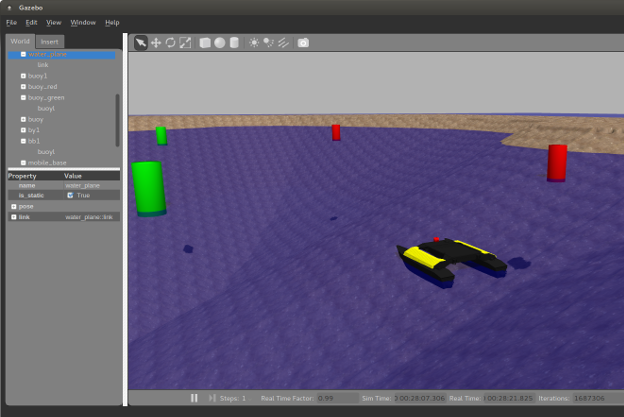
\includegraphics[width=.7\textwidth]{example.png}
  \caption{Ex0}
  \label{f:e0}
\end{figure}


\begin{enumerate}
\item {\bf Physics:} is important.To resolve collision, contact, and reaction forces among
\item {\bf Sensors:}
\end{enumerate}


\subsection{Virtual Robotics Competitions}


\begin{figure}[h]
  \centering
  \begin{subfigure}[t]{0.3\textwidth}
    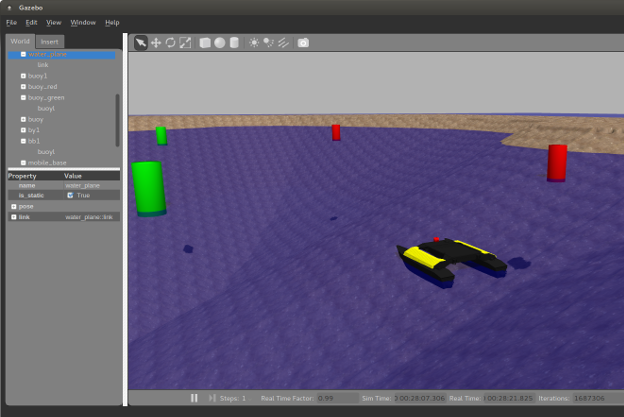
\includegraphics[width=\textwidth]{example.png}
    \caption{Ex1}
  \end{subfigure}
  ~
  \begin{subfigure}[t]{0.3\textwidth}
    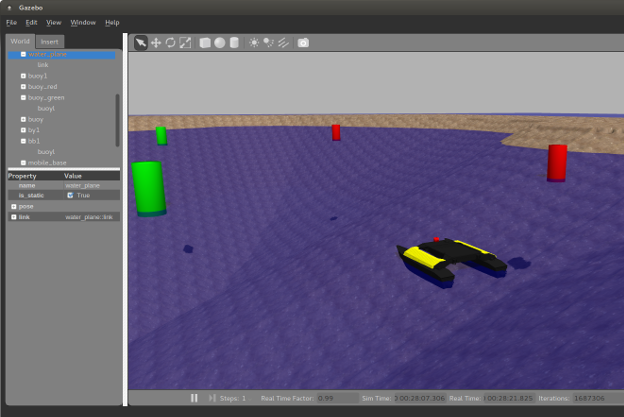
\includegraphics[width=\textwidth]{example.png}
    \caption{Ex2}
  \end{subfigure}
  ~
  \begin{subfigure}[t]{0.3\textwidth}
    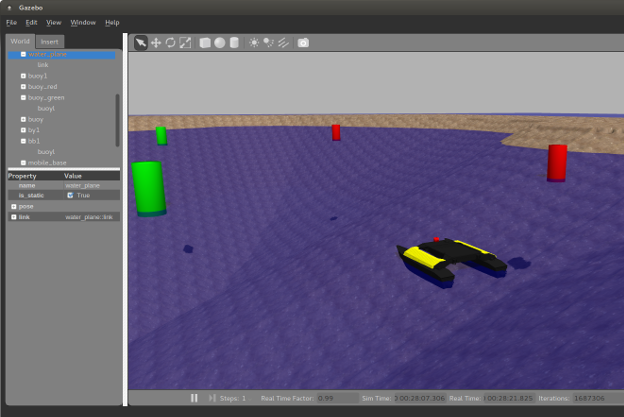
\includegraphics[width=\textwidth]{example.png}
    \caption{Ex3}
  \end{subfigure}\\
  ~
  \begin{subfigure}[t]{0.3\textwidth}
    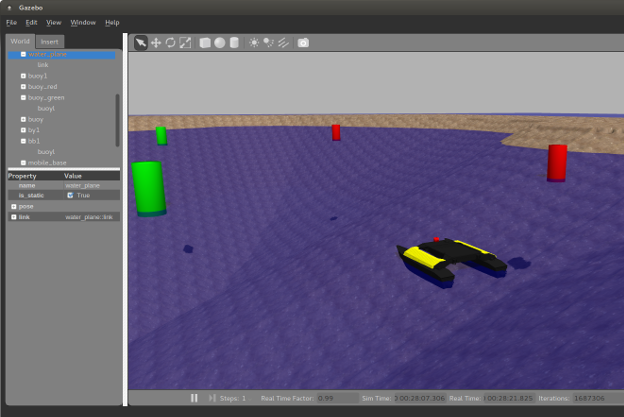
\includegraphics[width=\textwidth]{example.png}
    \caption{Ex4}
  \end{subfigure}
  ~
  \begin{subfigure}[t]{0.3\textwidth}
    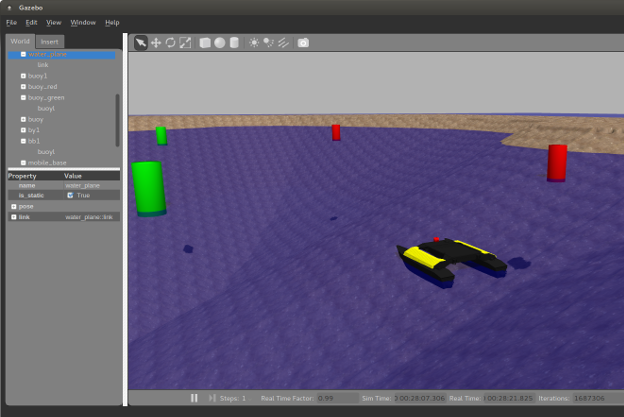
\includegraphics[width=\textwidth]{example.png}
    \caption{Ex5}
  \end{subfigure}
  ~
  \begin{subfigure}[t]{0.3\textwidth}
    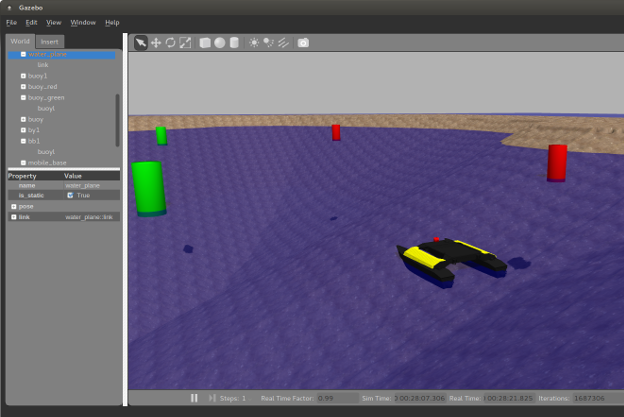
\includegraphics[width=\textwidth]{example.png}
    \caption{Ex6}
  \label{f:e1}
  \end{subfigure}
\end{figure}

\hlr{This is a red highlighted note.}

\begin{description}
\item[Extensible sensor modeling]: In addition to native sensor simulation, should afford the capability to extend existing sensing modalities to account for future applications.
\item[Multiple vehicles]: Should scale to multiple vehicles.
\end{description}

\section{Technical Approach}
Sed sem felis, luctus sit amet fermentum vulputate, laoreet vel massa. In hac habitasse platea dictumst. Praesent ac tincidunt arcu. Donec quis elementum sapien. Ut non odio elementum neque ullamcorper viverra consequat ut est. Etiam posuere lectus non felis pharetra, quis vestibulum quam semper. Praesent et tortor nec orci accumsan volutpat. Integer posuere lacus at nisi vulputate, eu tincidunt tellus facilisis.

\begin{figure}[htbp]
\begin{subfigure}[t]{0.65\textwidth}
  \centering
  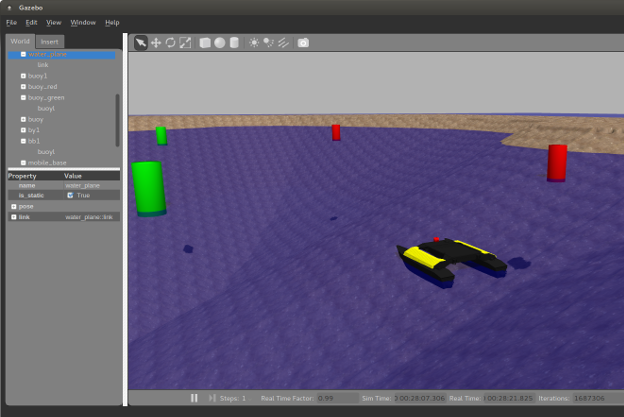
\includegraphics[width=0.99\linewidth]{example.png}
  \captionsetup{width=0.9\linewidth}
  \caption{ex7}
  \label{f:ex7}
\end{subfigure}
\begin{subfigure}[t]{0.35\textwidth}
  \centering
  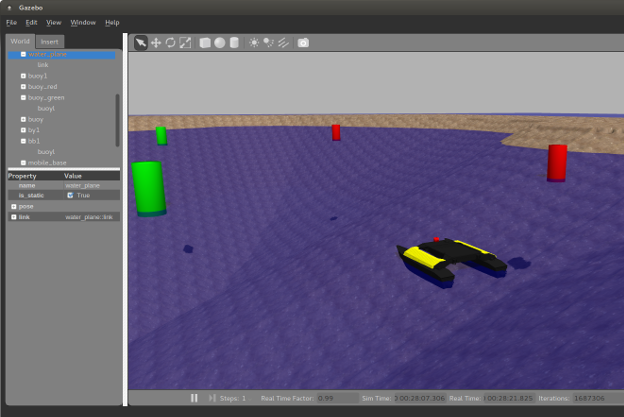
\includegraphics[width=0.99\linewidth]{example.png}
  \captionsetup{width=0.9\linewidth}
  \caption{ex8}
  \label{f:ex8}
\end{subfigure}
\caption{More examples.}
\label{f:more_ex}
\end{figure}

\section{Statement of Work}
The work can be nominally divided into three components: simulation development, hosting the VMRC and community support.  For each task the lead organization is identified ({\bf[NPS]} or {\bf[OSRF]}), but the tasks are will be executed collaboratively.

\newlist{sow}{enumerate}{10}
\setlist[sow]{label*=\textbf{\arabic*.},leftmargin=*}

\begin{sow}
\item Simulation Development Tasks:
  \begin{sow}
  \item Work with RobotX organizers and participants to specify the requirements of a simulation environment for the VMRC, including specifications of required and optional simulation components. {\bf[NPS]}
    \begin{sow}
    \item Document what middleware and interface software is in use by current teams, eg., ROS, MOOS, LCM, etc.  {\bf[NPS]}
    \item Identify high value Gazebo environmental extensions for maritime robotics (e.g., wave forcing, wind effects, acoustic sensing, etc.) based on development effort required and utility for maritime robotics development.  {\bf[NPS]}
    \end{sow}
  \item Develop new (or improve existing) software plugins for Gazebo to enable simulation of USV and UUV robotic platforms, including buoyancy, hydrodynamic and environment effects. {\bf[NPS]} with support by {\bf[OSRF]}
    \begin{sow}
      \item Generate platform-specific models, using these generic plugins, to replicate the dynamics of the WAM-V USV platform. {\bf[OSRF]}
      \item Generate platform-specific models, using these generic plugins, to replicate the dynamics of a common UUV platforms - model to be determined. {\bf[OSRF]}
    \end{sow}
  \item Create environment models to replicate typical USV and UUV missions, e.g., surface harbor navigation, large-area search, etc.  These models will be used as the basis for basic autonomy building blocks and automated tests in the virtual competition. {\bf[OSRF]}
  \end{sow}
\item Hosting Virtual RobotX Competition Tasks:
  \begin{sow}
  \item Design, test and document a single API for the virtual RobotX competition.  This API would provide a common interface to participants using a variety of robot middleware such as MOOS, ROS, LCM and custom solutions. {\bf[OSRF]}
  \item Create environment models to replicate a subset of the RobotX competition tasks amenable for competition challenges in the virtual competition. {\bf[OSRF]}
  \item Implement, document and maintain a cloud computing environment for the virtual RobotX competition in fall 2019. {\bf[OSRF]}
  \item Provide technical support during development, practice, dry-run and competition phasis of VMRC. {\bf[OSRF]}
  \end{sow}
  \item Community Support Tasks:
  \begin{sow}
    \item Participate in the December 2017 RobotX competitors meeting and lead the following activities:
      \begin{sow}
        \item A half-day ROS/Gazebo tutorial {\bf[NPS]}
        \item An overview of the VRMC concept and design discussion on the VRMC API. {\bf[OSRF]}
        \item A design exercise on generate concepts for VRMC tasks {\bf[NPS]}
        \end{sow}
      \item Attend the 2018 RobotX challenge to assist competitors preparing for the VRMC. \\ {\bf[OSRF]} and {\bf[NPS]}
      \item Collaborate with RobotX organizers and supporters as needed to implement the VRMC. \\ {\bf[OSRF]} and {\bf[NPS]}
  \end{sow}
\end{sow}

\section{Schedule}
The following schedule assumes support for development can begin 1 December 2017.
\begin{description}
\item[December 2017:] RobotX competitor's meeting.  Meet with competitors and organizers to develop use-cases for use in API and virtual challenge requirements.  Hold half-day tutorial.
  \begin{itemize}
  \item Collect information on use-cases for existing teams.  What software tools and development support do they current use?  What capabilities will be required to host successful competition?
  \end{itemize}
\item[March 2018:] First draft of requirements for simulation development, VMRC tasks and API.  Internal review of specifications with NPS, OSRF, ONR and other stakeholders.
  \begin{itemize} 
  \item Identify basic autonomy tasks to be the source for VMRC task descriptions
  \end{itemize}
\item[June 2018:] Prototype development tools (Gazebo plugins, worlds and models) are released as actively developed tools for internal and external testing.
\item[September 2018:] Internal review of rules, requirements and API.  Completed testing of development tools (plugins, worlds, models, etc.)
\item[December 2018:] Maritime RobotX Challenge.  
  \begin{itemize}
  \item Release draft rules and requirements for RobotX Virtual Challenge.
  \item Registration for VMRC
  \end{itemize}
\item[March 2019:] Prototype of fully functional simulation environment, API and technical guide for participants.
  \begin{itemize}
  \item Begin internal testing 
  \end{itemize}
\item[June 2019:] Final competition specifications.
  \begin{itemize}
  \item Release of final rules, scenarios and API.  Teams can continue building based on final specifications.
  \end{itemize}  
\item[November 2019:] Cloud environment open for team practice
  \begin{itemize}
  \item Teams can provision and run cloud-based tasks similar, but not identical, to competition tasks.  Allows teams to test and verify integration with challenge environment with asynchronous support.
  \end{itemize}
\item[December 2019:] Virtual Maritime RobotX Challenge (VMRC) Event
  \begin{itemize}
  \item Dry Run: One day of teams running on full cloud environment with 24 hour support.
  \item Competition: Two days for teams to run N runs of M tasks with scoring and 24 hour support.
  \end{itemize}
\end{description}



\newpage
\setcounter{page}{1}
\bibliographystyle{ieee/IEEEtran}
% argument is your BibTeX string definitions and bibliography database(s)
\bibliography{refs}

\end{document}
